\documentclass{standalone}
\usepackage{tikz}
\usetikzlibrary{positioning}
\usetikzlibrary {shapes.geometric}
\usetikzlibrary {shapes.symbols}
\pagestyle{empty}

\begin{document}

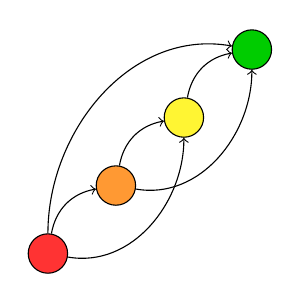
\begin{tikzpicture}
    [elementRed/.style={circle, draw=black, fill=red!80, inner sep=0pt, minimum size=5mm},
     elementOrange/.style={circle, draw=black, fill=orange!80, inner sep=0pt, minimum size=5mm},
     elementYellow/.style={circle, draw=black, fill=yellow!80, inner sep=0pt, minimum size=5mm},
     elementGreen/.style={circle, draw=black, fill=black!20!green, inner sep=0pt, minimum size=5mm},
    ]

    \node[elementRed] (redDot) [] {};
    \node[elementOrange] (orangeDot) [above right=5mm and 5mm of redDot] {}
        edge [<-, out=190, in=80] (redDot);
    \node[elementYellow] (yellowDot) [above right=5mm and 5mm of orangeDot] {}
        edge [<-, out=190, in=80] (orangeDot)
        edge [<-, out=270, in=350] (redDot);
    \node[elementGreen] (greenDot) [above right=5mm and 5mm of yellowDot] {}
        edge [<-, out=190, in=80] (yellowDot)
        edge [<-, out=270, in=350] (orangeDot)
        edge [<-, out=170, in=90] (redDot);

\end{tikzpicture}

\end{document}